% Options for packages loaded elsewhere
\PassOptionsToPackage{unicode}{hyperref}
\PassOptionsToPackage{hyphens}{url}
\PassOptionsToPackage{space}{xeCJK}
\documentclass[
  10pt,
]{article}
\usepackage{xcolor}
\usepackage[margin=0.8in]{geometry}
\usepackage{amsmath,amssymb}
\setcounter{secnumdepth}{-\maxdimen} % remove section numbering
\usepackage{iftex}
\ifPDFTeX
  \usepackage[T1]{fontenc}
  \usepackage[utf8]{inputenc}
  \usepackage{textcomp} % provide euro and other symbols
\else % if luatex or xetex
  \usepackage{unicode-math} % this also loads fontspec
  \defaultfontfeatures{Scale=MatchLowercase}
  \defaultfontfeatures[\rmfamily]{Ligatures=TeX,Scale=1}
\fi
\usepackage{lmodern}
\ifPDFTeX\else
  % xetex/luatex font selection
  \setmainfont[]{Arial}
  \ifXeTeX
    \usepackage{xeCJK}
    \setCJKmainfont[]{Microsoft YaHei}
  \fi
  \ifLuaTeX
    \usepackage[]{luatexja-fontspec}
    \setmainjfont[]{Microsoft YaHei}
  \fi
\fi
% Use upquote if available, for straight quotes in verbatim environments
\IfFileExists{upquote.sty}{\usepackage{upquote}}{}
\IfFileExists{microtype.sty}{% use microtype if available
  \usepackage[]{microtype}
  \UseMicrotypeSet[protrusion]{basicmath} % disable protrusion for tt fonts
}{}
\makeatletter
\@ifundefined{KOMAClassName}{% if non-KOMA class
  \IfFileExists{parskip.sty}{%
    \usepackage{parskip}
  }{% else
    \setlength{\parindent}{0pt}
    \setlength{\parskip}{6pt plus 2pt minus 1pt}}
}{% if KOMA class
  \KOMAoptions{parskip=half}}
\makeatother
\usepackage{longtable,booktabs,array}
\newcounter{none} % for unnumbered tables
\usepackage{calc} % for calculating minipage widths
% Correct order of tables after \paragraph or \subparagraph
\usepackage{etoolbox}
\makeatletter
\patchcmd\longtable{\par}{\if@noskipsec\mbox{}\fi\par}{}{}
\makeatother
% Allow footnotes in longtable head/foot
\IfFileExists{footnotehyper.sty}{\usepackage{footnotehyper}}{\usepackage{footnote}}
\makesavenoteenv{longtable}
\usepackage{graphicx}
\makeatletter
\newsavebox\pandoc@box
\newcommand*\pandocbounded[1]{% scales image to fit in text height/width
  \sbox\pandoc@box{#1}%
  \Gscale@div\@tempa{\textheight}{\dimexpr\ht\pandoc@box+\dp\pandoc@box\relax}%
  \Gscale@div\@tempb{\linewidth}{\wd\pandoc@box}%
  \ifdim\@tempb\p@<\@tempa\p@\let\@tempa\@tempb\fi% select the smaller of both
  \ifdim\@tempa\p@<\p@\scalebox{\@tempa}{\usebox\pandoc@box}%
  \else\usebox{\pandoc@box}%
  \fi%
}
% Set default figure placement to htbp
\def\fps@figure{htbp}
\makeatother
\setlength{\emergencystretch}{3em} % prevent overfull lines
\providecommand{\tightlist}{%
  \setlength{\itemsep}{0pt}\setlength{\parskip}{0pt}}
\usepackage{bookmark}
\IfFileExists{xurl.sty}{\usepackage{xurl}}{} % add URL line breaks if available
\urlstyle{same}
\hypersetup{
  hidelinks,
  pdfcreator={LaTeX via pandoc}}

\author{}
\date{}

\usepackage{float}
\begin{document}

\section{模型训练进展报告}\label{ux6a21ux578bux8badux7ec3ux8fdbux5c55ux62a5ux544a}

\href{training-progress.en.md}{English} \textbar{} 中文

数据核对日期：2026-11-12。依据项目内已保存的正式训练和模型验证记录。

\subsection{训练状态与记录}\label{ux8badux7ec3ux72b6ux6001ux4e0eux8bb0ux5f55}

{\def\LTcaptype{none} % do not increment counter
\begin{longtable}[]{@{}
  >{\raggedright\arraybackslash}p{(\linewidth - 8\tabcolsep) * \real{0.1667}}
  >{\raggedright\arraybackslash}p{(\linewidth - 8\tabcolsep) * \real{0.1667}}
  >{\raggedleft\arraybackslash}p{(\linewidth - 8\tabcolsep) * \real{0.2222}}
  >{\raggedleft\arraybackslash}p{(\linewidth - 8\tabcolsep) * \real{0.2222}}
  >{\raggedleft\arraybackslash}p{(\linewidth - 8\tabcolsep) * \real{0.2222}}@{}}
\toprule\noalign{}
\begin{minipage}[b]{\linewidth}\raggedright
任务
\end{minipage} & \begin{minipage}[b]{\linewidth}\raggedright
模型
\end{minipage} & \begin{minipage}[b]{\linewidth}\raggedleft
训练 / 验证图像
\end{minipage} & \begin{minipage}[b]{\linewidth}\raggedleft
已完成
\end{minipage} & \begin{minipage}[b]{\linewidth}\raggedleft
训练 step
\end{minipage} \\
\midrule\noalign{}
\endhead
\bottomrule\noalign{}
\endlastfoot
青光眼 A & EfficientNet-B0 & 10,354 / 1,190 & 20 / 20 epoch & 12,960 \\
青光眼 B（候选） & ResNet50 & 10,354 / 1,190 & 20 / 20 epoch & 12,960 \\
formal\_v3 图像质量蒸馏 & EfficientNet-B0 & 12,147 / 1,642 & 20 / 20 epoch & 15,200 \\
EyeQ 质量模型 & EfficientNet-B0 & 4,722 / 616 & 20 / 20 epoch & 5,920 \\
\end{longtable}
}

两条训练队列的状态文件均记录为 completed。每组 \texttt{steps.jsonl} 保存每个训练 batch 的损失、步数和梯度信息；\texttt{epochs.jsonl} 保存每轮验证结果，\texttt{best.pt} 和 \texttt{last.pt} 保存模型检查点。四组日志步数连续，训练损失值均有限。图中的训练损失是每个 epoch 内所记录 batch 损失的算术平均，而非逐样本加权平均。formal\_v3 日志的 epoch 从 0 开始，图表统一标成第 1--20 轮；EyeQ 验证日志本身从 1 开始。

\begin{figure}[H]
\centering
\pandocbounded{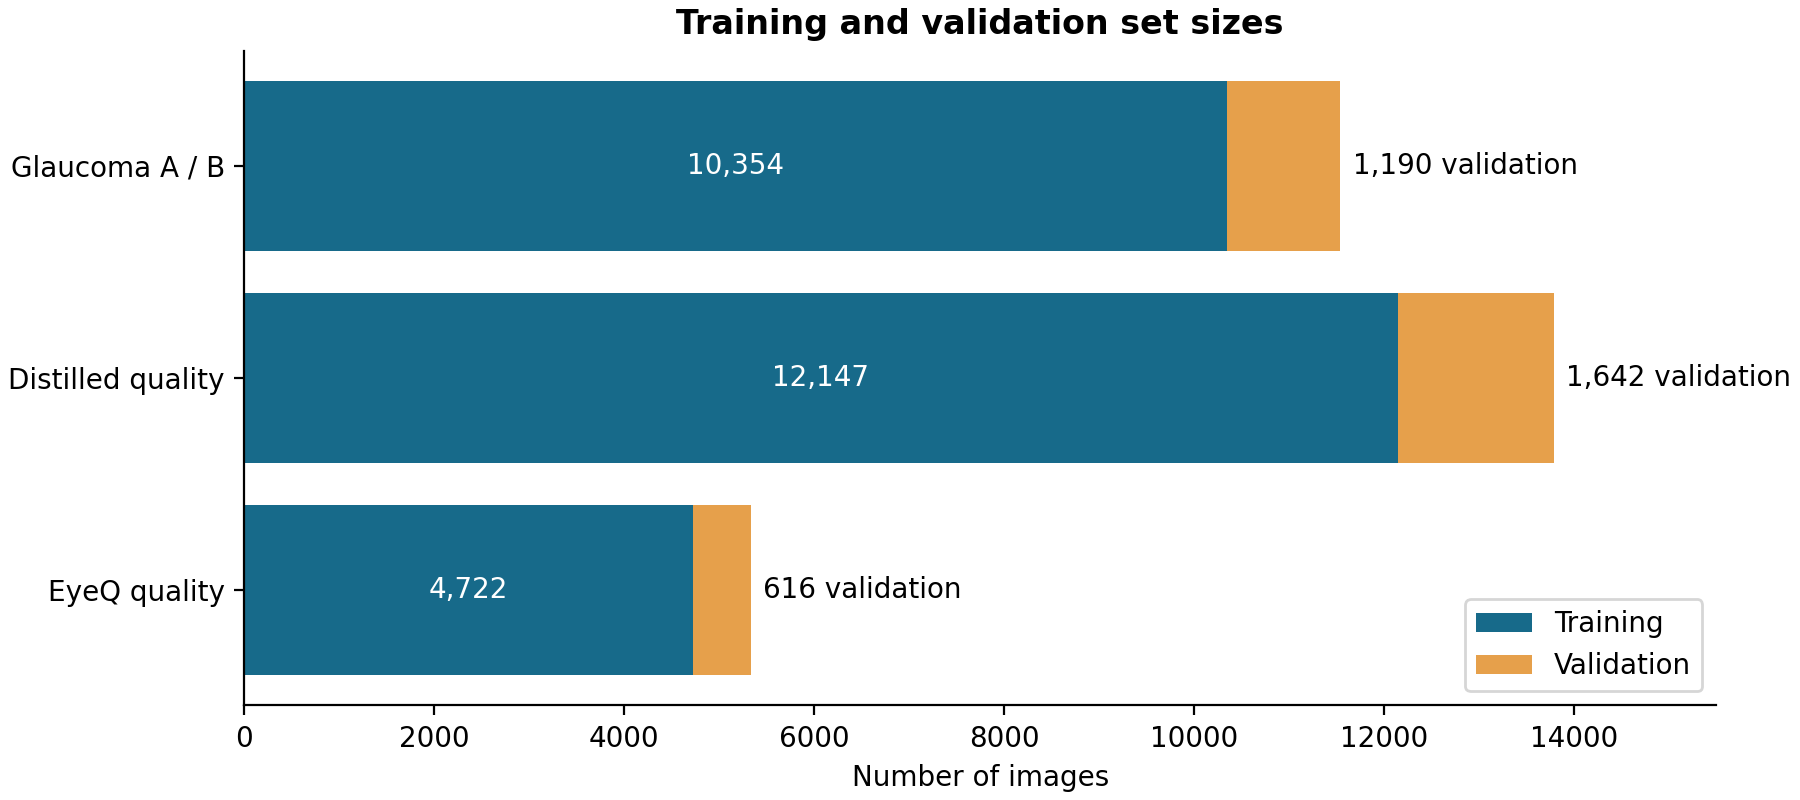
\includegraphics[keepaspectratio,alt={训练与验证集规模}]{07_dataset_sizes.png}}
\caption{训练与验证集规模}
\end{figure}

上图显示各模型使用的图像数量。青光眼 A 和 B 使用相同的数据划分。一个 epoch 指模型遍历一轮训练数据；一个 step 指使用一批图像完成一次训练。

\begin{figure}[H]
\centering
\pandocbounded{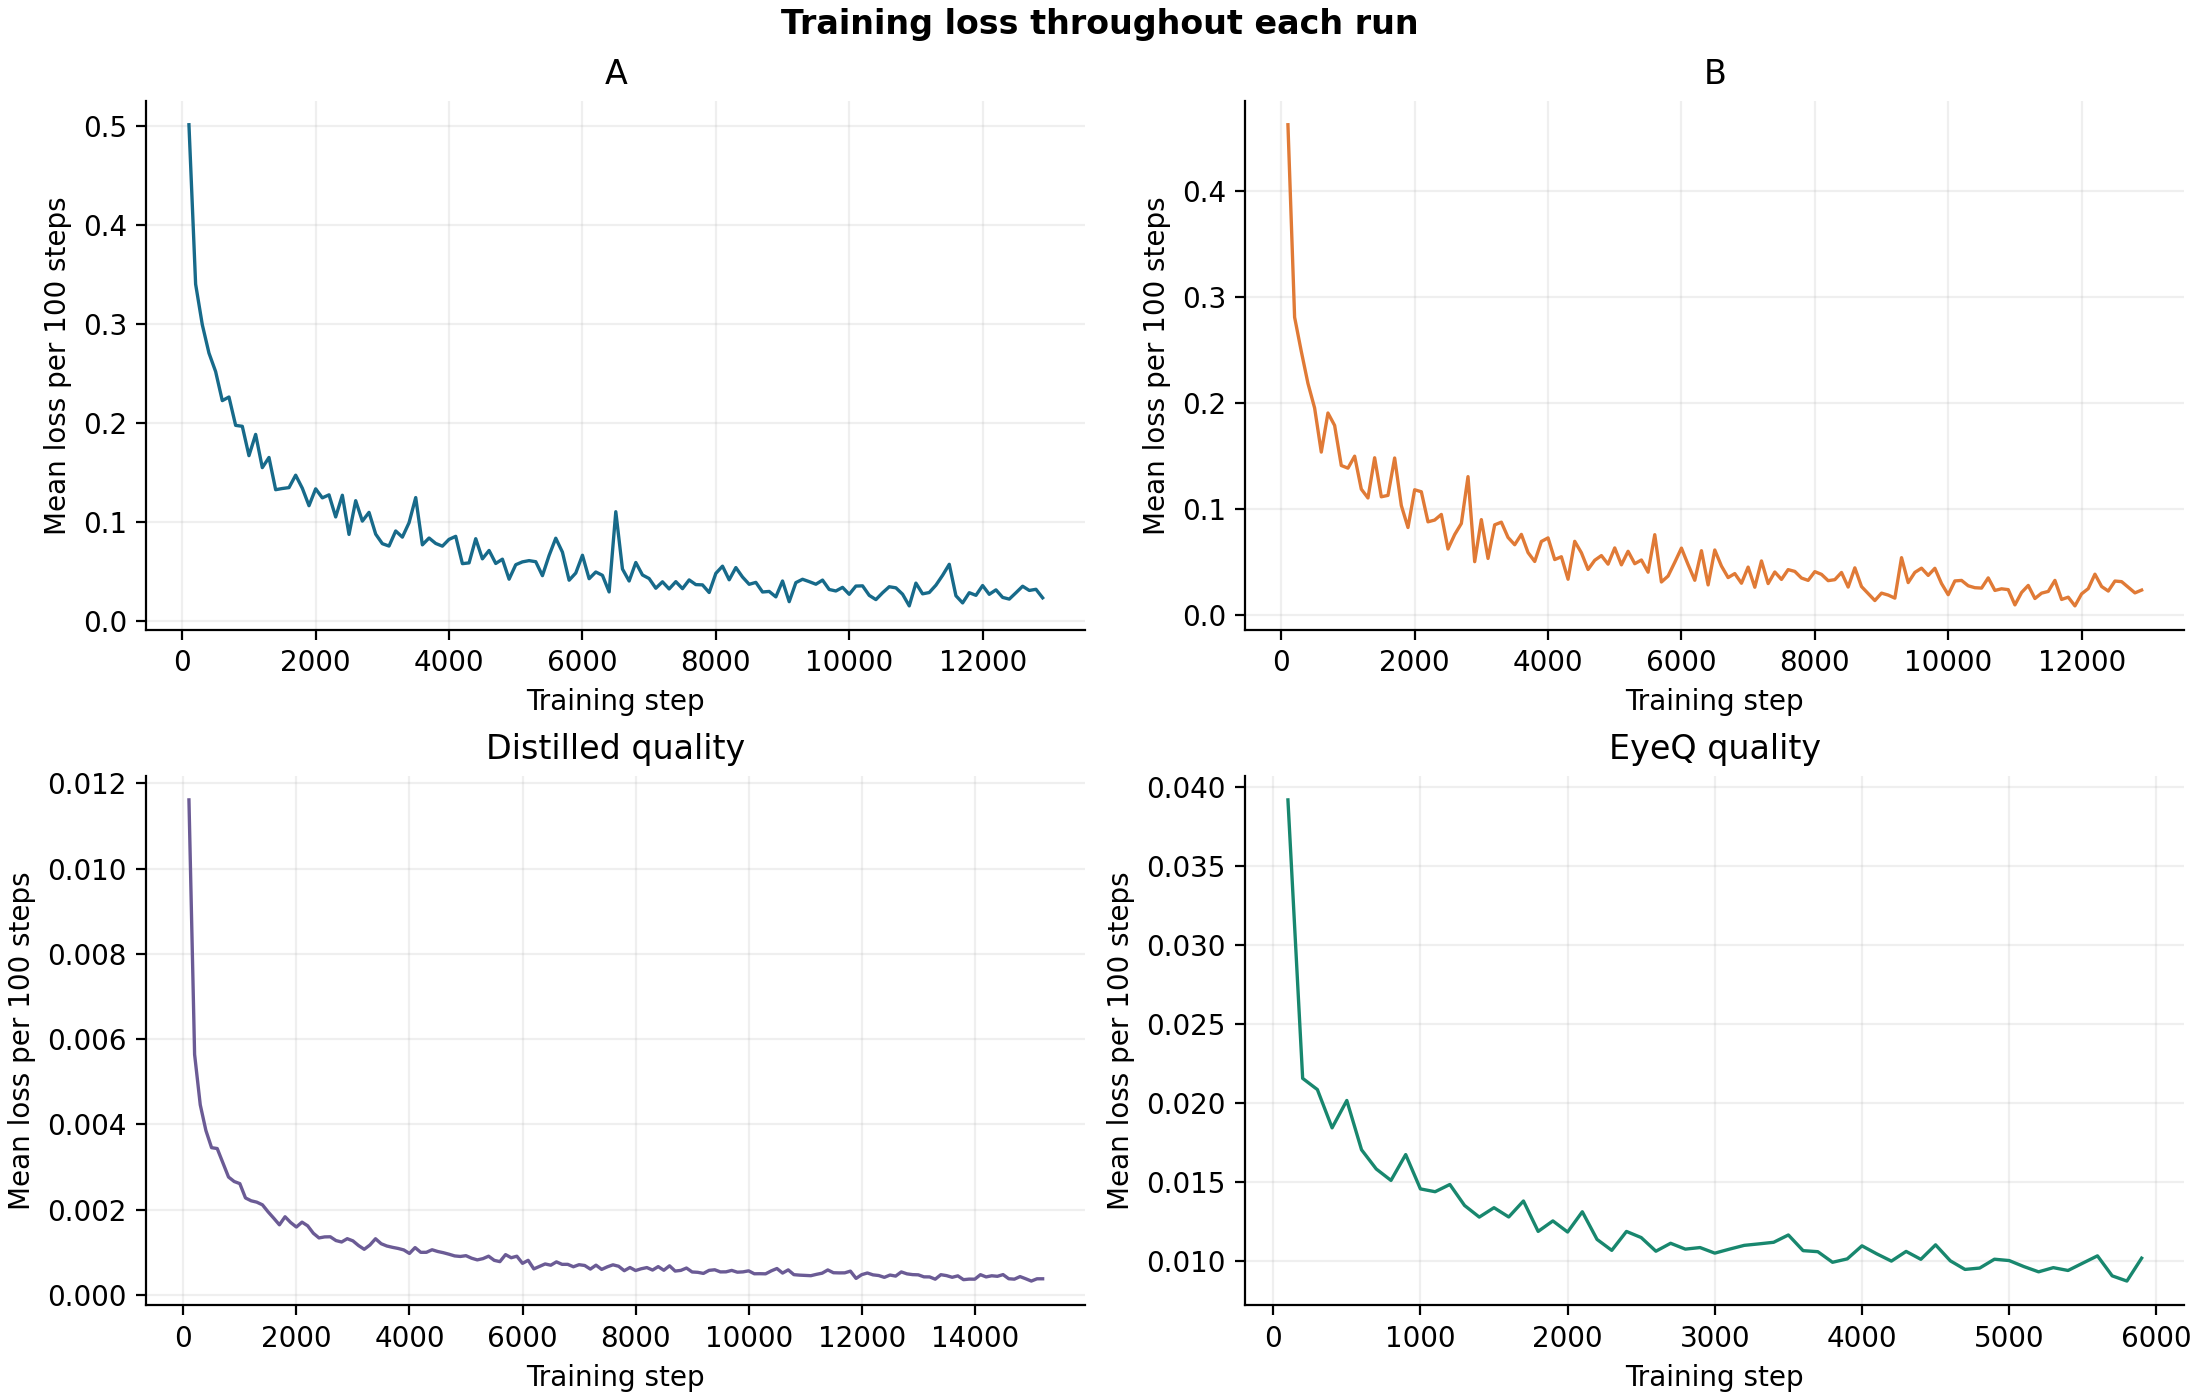
\includegraphics[keepaspectratio,alt={逐步训练损失}]{04_step_loss.png}}
\caption{逐步训练损失}
\end{figure}

为便于观察，图中每个点是连续 100 个训练步骤的平均损失。损失越低表示模型在该批数据上与训练目标的差异越小。

\subsection{青光眼模型}\label{ux9752ux5149ux773cux6a21ux578b}

\begin{figure}[H]
\centering
\pandocbounded{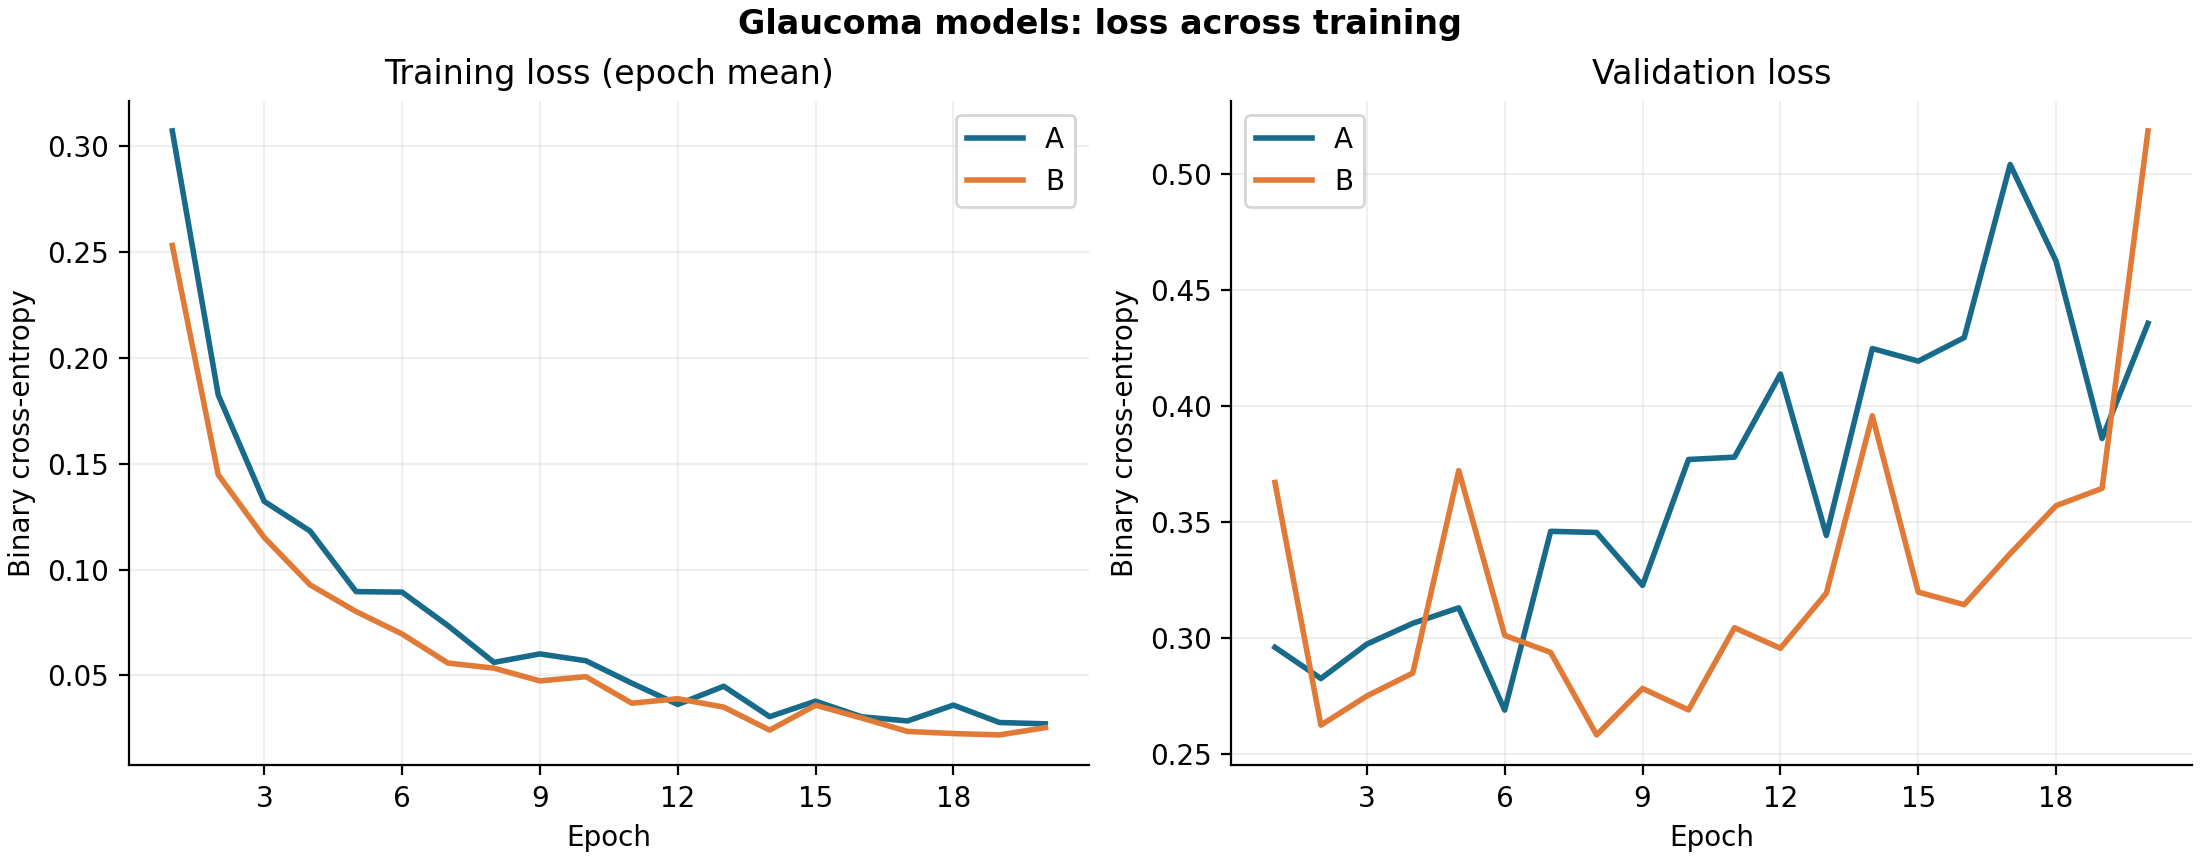
\includegraphics[keepaspectratio,alt={训练和验证损失}]{01_glaucoma_loss.png}}
\caption{训练和验证损失}
\end{figure}

A 的训练损失均值从第 1 轮的 0.307 降至第 20 轮的 0.027；B 从 0.253 降至 0.025。对应的整体验证损失从 0.296 升至 0.435（A），从 0.367 升至 0.518（B）。训练损失下降而末轮验证损失高于首轮，提示应关注过拟合或概率校准问题。

\begin{figure}[H]
\centering
\pandocbounded{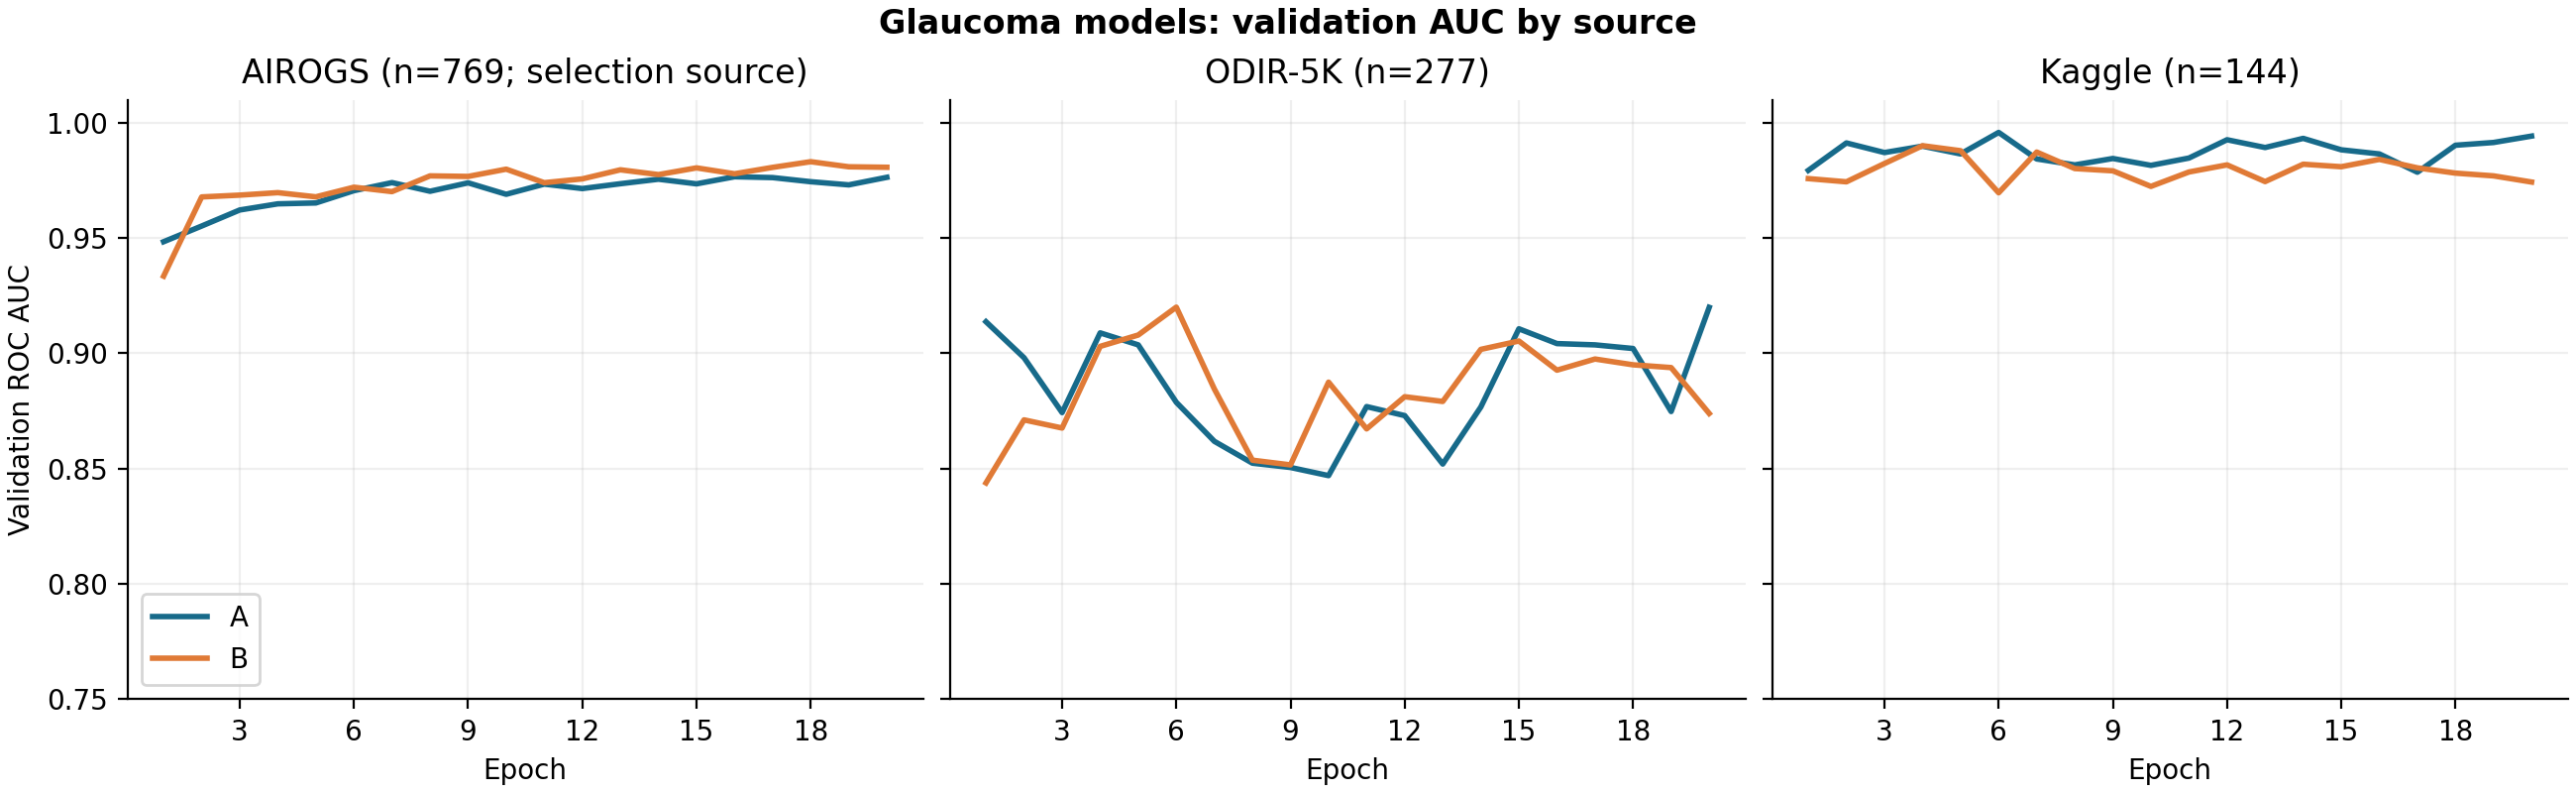
\includegraphics[keepaspectratio,alt={验证集分数据源 AUC}]{02_glaucoma_auc.png}}
\caption{验证集分数据源 AUC}
\end{figure}

AUC 衡量模型将阳性样本排在阴性样本之前的能力。训练配置使用 AIROGS 验证子集的 AUC 选择最佳检查点（769 张）。A 最佳为第 16 轮 AUC \textbf{0.9766}，B 最佳为第 18 轮 \textbf{0.9831}；第 20 轮分别为 0.9764 和 0.9807。其他来源验证集分别为 ODIR-5K 277 张、Kaggle 144 张。

疾病模型日志没有逐轮保存准确率，只保存验证损失和各来源 AUC。\texttt{validation\_predictions.csv} 在每轮验证时覆盖，因此对应最后一次验证，不能据此重建每一轮或最佳检查点的准确率。

\subsection{图像质量模型}\label{ux56feux50cfux8d28ux91cfux6a21ux578b}

\begin{figure}[H]
\centering
\pandocbounded{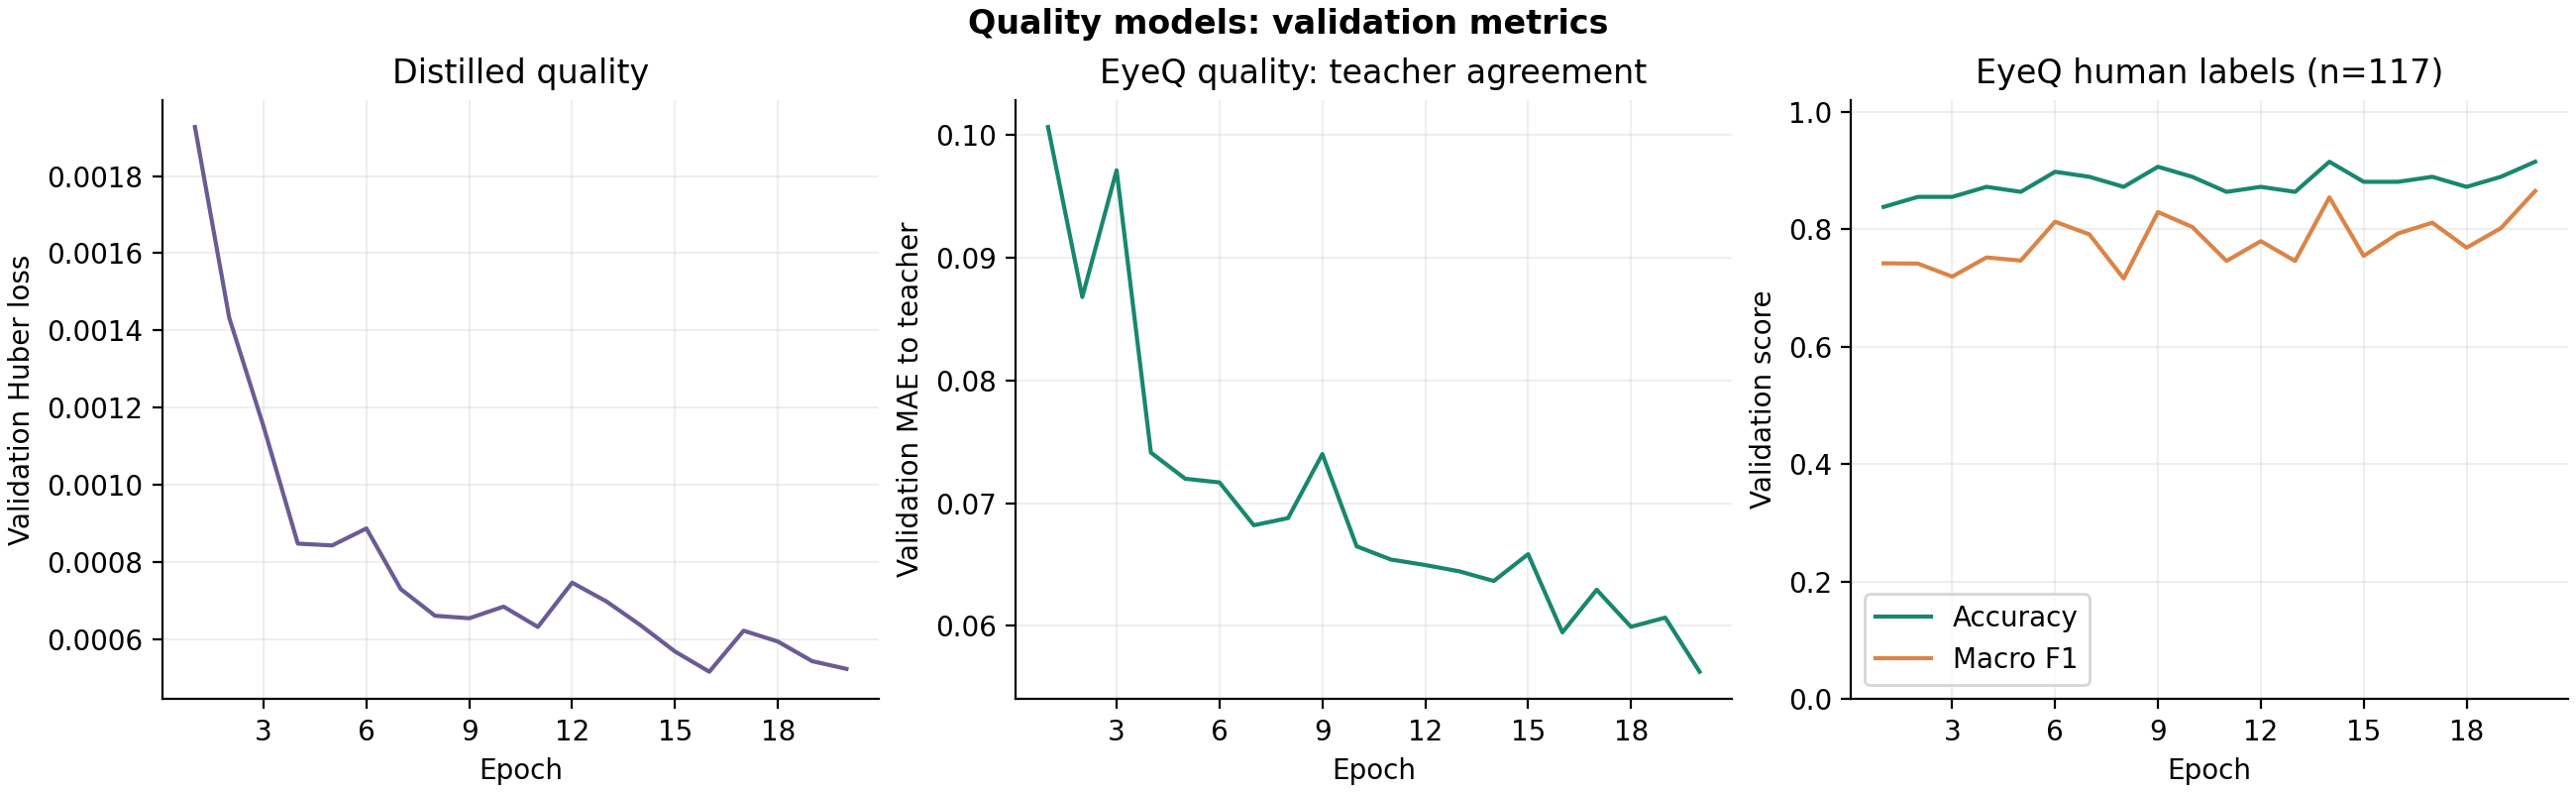
\includegraphics[keepaspectratio,alt={质量模型验证指标}]{03_quality_validation.png}}
\caption{质量模型验证指标}
\end{figure}

\begin{itemize}
\tightlist
\item
  formal\_v3 质量蒸馏模型的验证 Huber loss 从 0.001927 降至 0.000524，最低为第 16 轮的 0.000517。验证目标为教师模型评分。
\item
  独立 EyeQ 质量模型使用 616 张验证图像，其中 117 张有 EyeQ 三档人工标签。由每轮混淆矩阵计算，准确率从第 1 轮 \textbf{83.8\%（98/117）}升至第 20 轮 \textbf{91.5\%（107/117）}；末轮 macro-F1 为 \textbf{0.865}。
\item
  EyeQ 的最佳检查点按教师 Huber loss 与人工标签序数损失组成的选择损失确定。按该规则选择的第 17 轮准确率为 \textbf{88.9\%（104/117）}、macro-F1 为 \textbf{0.811}。
\end{itemize}

\begin{figure}[H]
\centering
\pandocbounded{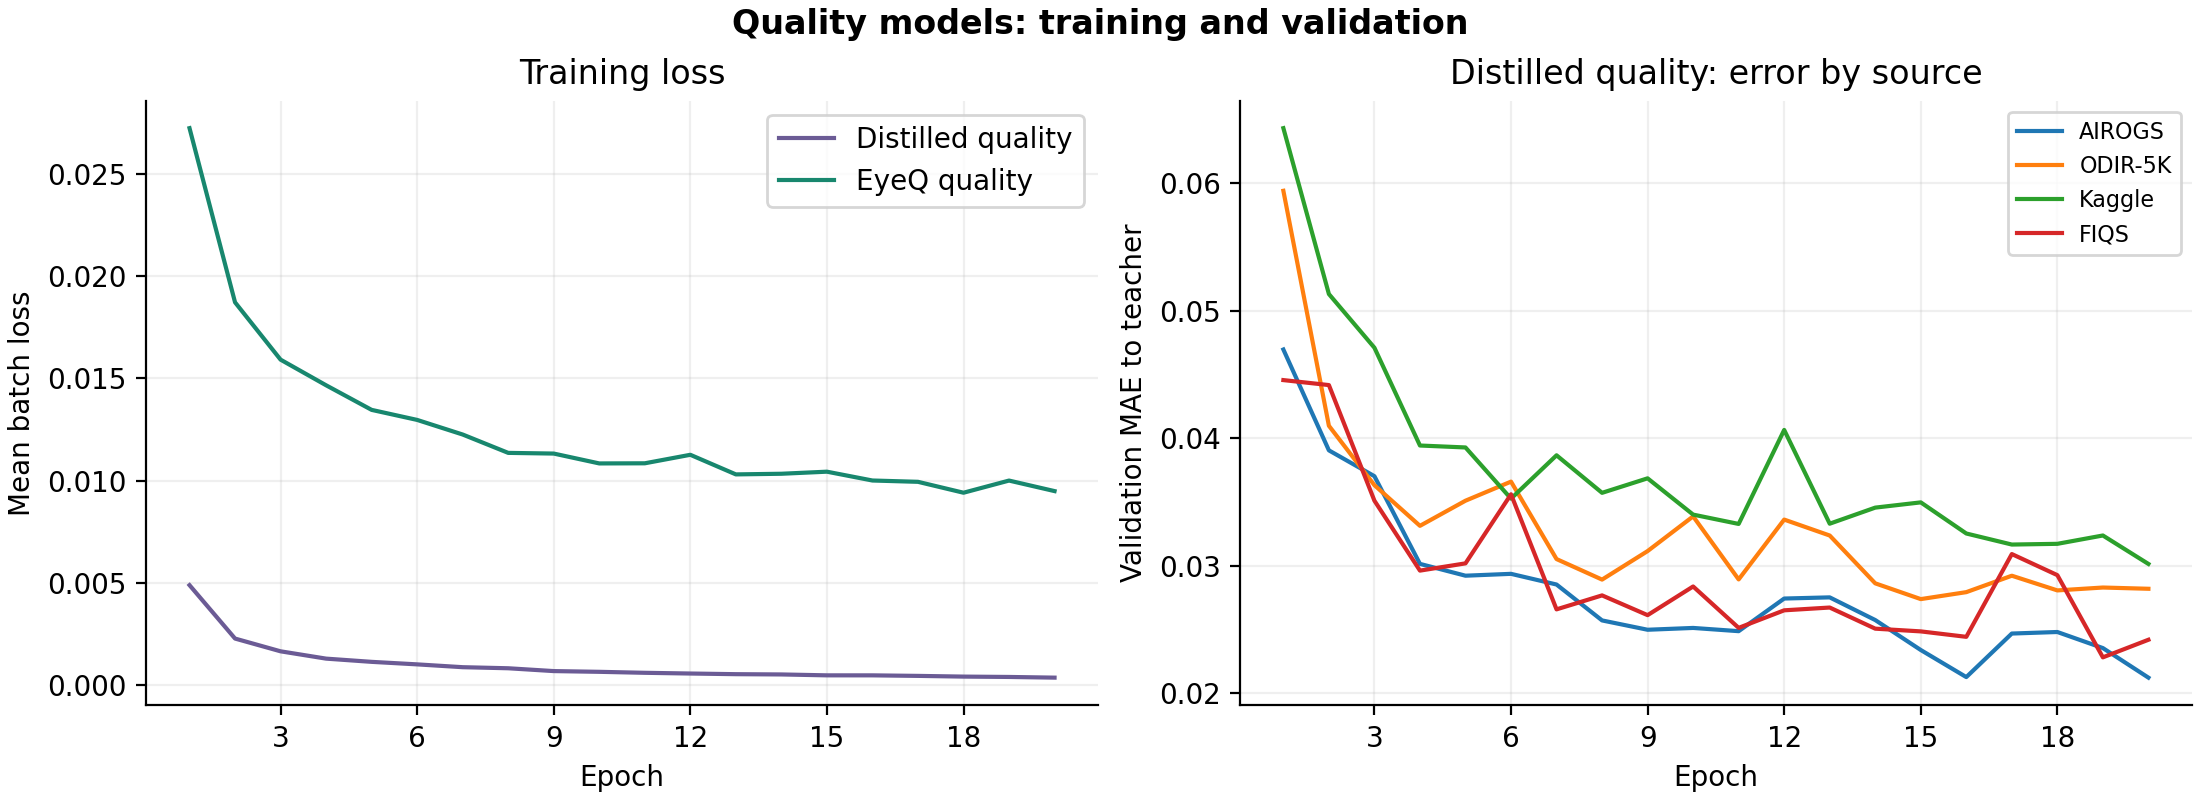
\includegraphics[keepaspectratio,alt={质量模型补充曲线}]{05_quality_detail.png}}
\caption{质量模型补充曲线}
\end{figure}

左图展示两种质量模型各自的训练损失。右图按图像来源展示原质量模型与教师评分的平均绝对误差（MAE），数值越低表示越接近教师评分。

\begin{figure}[H]
\centering
\pandocbounded{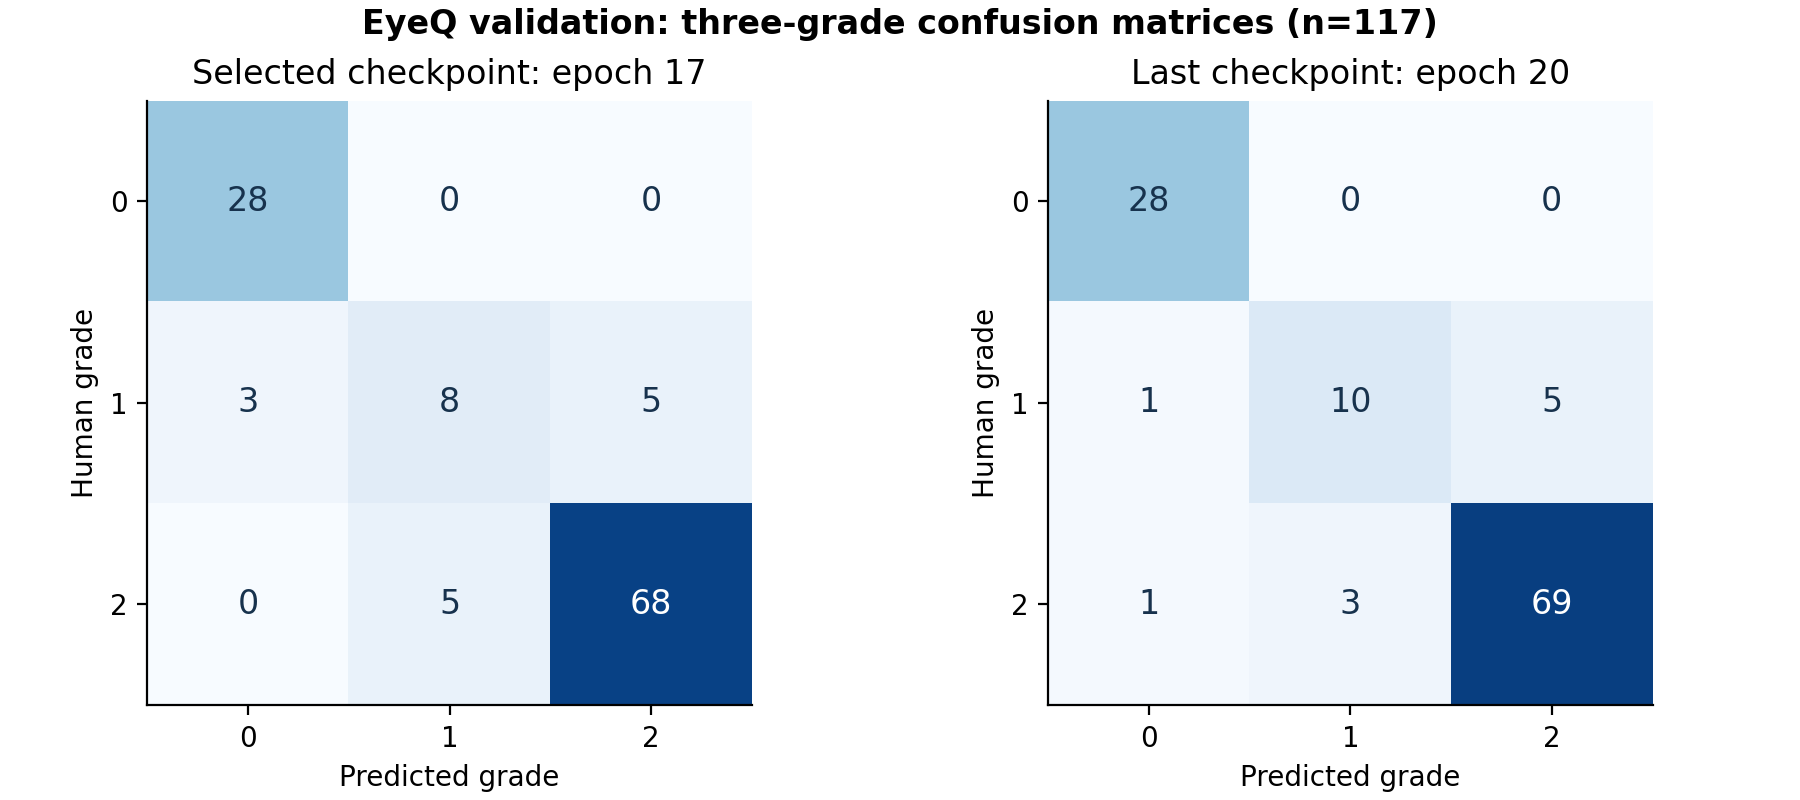
\includegraphics[keepaspectratio,alt={EyeQ 验证混淆矩阵}]{06_eyeq_confusion.png}}
\caption{EyeQ 验证混淆矩阵}
\end{figure}

矩阵的行表示人工质量等级，列表示模型预测等级；对角线上的数字是预测正确的图像数。第 17 轮是按预先设定的选择损失确定的检查点，第 20 轮是最后一轮。Macro-F1 是分别计算各等级的 F1 分数后取平均，用于同时观察各等级的表现。

\subsection{数据来源与图表生成}\label{ux6570ux636eux6765ux6e90ux4e0eux56feux8868ux751fux6210}

数据来源：\texttt{runs/formal\_v3/\{glaucoma\_a,glaucoma\_b\_candidate,quality\_student\}/\{steps,epochs\}.jsonl}、\texttt{runs/eyeq\_quality\_v1/quality\_student/\{steps,epochs\}.jsonl}，以及对应 \texttt{config.json}、\texttt{run\_summary.json} 和队列 \texttt{status.json}。重新生成图表：运行本目录的 \texttt{plot\_training.py}，需要 Python 和 matplotlib。图表使用随报告保存的 \texttt{chart\_data.json}；其中只包含训练步数、损失和汇总验证指标，不包含图像或样本身份。

\end{document}
